\documentclass{beamer}

\usepackage[utf8]{inputenc}
\usepackage[frenchb]{babel}
\usepackage[T1]{fontenc}
\usepackage{graphicx}
\usepackage{listings}
\usepackage{color}
\usepackage{mathtools}

\usetheme{Warsaw}
 
\begin{document}
 


\begin{frame}
\frametitle{$\lambda$-calcul}
\framesubtitle{Grammaire}

\begin{columns}

\begin{column}{5cm}
\begin{itemize}
\item $\lambda$ = ``l''
\item arguments séparés du corps par ``.''
\item plusieurs arguments, curryfiés plus tard
\item application associative gauche (xxx => (x x) x)
\end{itemize}
\end{column}

\begin{column}{5cm}
\textbf{Exemples :}
\linebreak
\linebreak
\textit{- lxy.y x}
\linebreak
\textit{- (lx.xx)(lx.xx)}
\linebreak
\textit{- abc}
\end{column}

\end{columns}

\end{frame}

\begin{frame}
\frametitle{$\lambda$-calcul}
\framesubtitle{Modélisation}

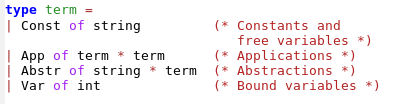
\includegraphics{lambda2.png}

\end{frame}

\begin{frame}
\frametitle{$\lambda$-calcul}
\framesubtitle{Indices de \textit{Bruijn}}

Variables liées codées par un entier.

\medskip

Valeur de cet entier = indice de l'abstraction en remontant l'arbre

\bigskip

\begin{columns}
\begin{column}{5cm}
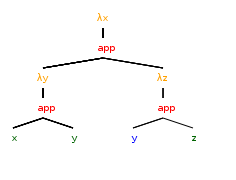
\includegraphics{lambda1.png}
\end{column}

\begin{column}{5cm}
Occurences liées :
\begin{itemize}
\item x <=> 1
\item y <=> 0
\item z <=> 0
\end{itemize}
\end{column}
\end{columns}


\end{frame}

\begin{frame}
\frametitle{$\lambda$-calcul}
\framesubtitle{$\alpha$-conversion}

\begin{columns}
\begin{column}{5cm}
\begin{itemize}
\item Changer le nom des variables liées pour éviter les ambiguïtés.
\item Ambiguïté quand il y a 2 abstractions de même argument dans la même branche.
\end{itemize}
\end{column}

\begin{column}{5cm}
\begin{center}
\textit{lx.(lx.x(lx.x))x}

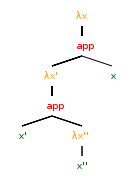
\includegraphics{lambda3.png}
\end{center}
\end{column}
\end{columns}

\end{frame}

\begin{frame}
\frametitle{$\lambda$-calcul}
\framesubtitle{$\beta$-réduction (1)}

Une seule règle de réduction :

\medskip

\textbf{($\lambda$x.M) N  -> B[N/x]}

\medskip

Substitution du paramètre par l'argument grâce aux indices de \textit{Bruijn}.

\end{frame}

\begin{frame}
\frametitle{$\lambda$-calcul}
\framesubtitle{$\beta$-réduction (2)}

Dans la formule :
\medskip
\textbf{($\lambda$x.\textcolor[rgb]{1,0,0}{M}) \textcolor[rgb]{0,0,1}{N}  -> B[\textcolor[rgb]{0,0,1}{N}/x]}

Faut-il évaluer d'abord \textcolor[rgb]{0,0,1}{N} (l'argument) ou \textcolor[rgb]{1,0,0}{M} (le corps de la fonction) ?

\bigskip

2 stratégies ont été implémentées :

\begin{itemize}
\item \textit{call-by-name} : On évalue d'abord le corps de la fonction.
\item \textit{call-by-value} : On évalue d'abord l'argument.
\end{itemize}

\end{frame}

\end{document}
